\section{Bottom up Pipeline}

The 'Top-Down' approach is great at allowing us to probe into the overall response of a deep-learning model. 
However to allow a more granular insight, we device pipeline model that works on selective obfuscation. 
The over all architecture of the pipeline can be see in figure \ref{fig:bottomup}. 
 \begin{figure*}[ht]
	\centering
	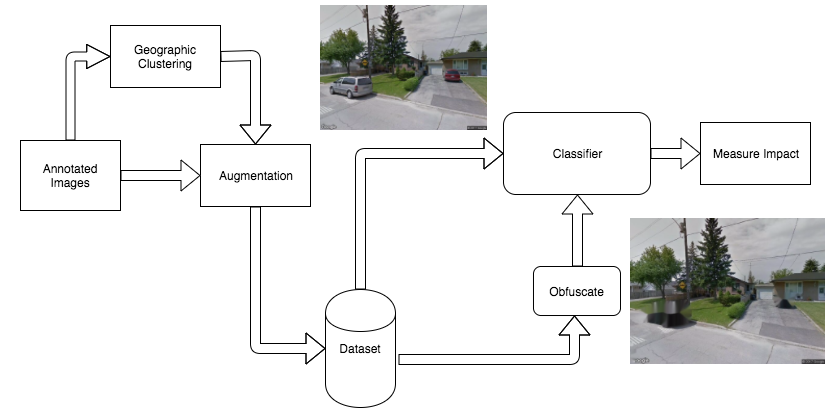
\includegraphics[width=1.5\columnwidth]{Plot/BottomupPipeline.png}
	\caption{Process pipeline for the "Bottom Up" approach for explainability}
	\label{fig:bottomup}
\end{figure*}

As seen from the figure, the preprocessing parts are reused from the 'top-down' approach. 
This pipeline does not employ the complex activation maximization approach, which helps us to 
transform images from one class to another, but employs a simpler method. As the aim of this approach
is to get a more granular understanding of what objects give rise to 